\documentclass[12pt]{article}
\usepackage[utf8]{inputenc}  
\usepackage[francais]{babel}  
\usepackage{graphicx}
\usepackage{url}
\usepackage[hidelinks,breaklinks]{hyperref}
\usepackage{breakurl}

\input{vc.tex}
                            
\begin{document} 
	\title{Mémoire}             
	\author{
		David Cheminade
		\and
		Guillaume Desbieys
		\and
		Quentin Michaud
		\and
		Hubert Mondon
	}                       
	\date{}
	\maketitle{}                

	\let\thefootnote\relax
	\footnotetext{Revision~\GITAbrHash, \GITAuthorDate.}             

	\clearpage
	\clearpage
	
	\section*{Resume}
	
	\paragraph{}
	Notre projet consiste à réaliser un moteur de règles pour le jeu de la guerre de Debord et à mettre en place un 
	évaluateur statique permettant de calculer les informations brutes nécessaires à une éventuelle future prise de décision.
	L'utilisateur peut fournir une situation de jeu sous forme de fichier ASCII et notre programme se chargera d'afficher 
	cette situation en y appliquant les diverses règles pour les calculs des zones d'influence et des potentiels offensifs et défensifs.
	L'objectif de ce projet est donc de créer une base solide qui permettra par la suite d'implémenter un moteur 
	décisionnel qui se base sur nos données statiques pour ses divers calculs.
	
	
	\clearpage
	
	\tableofcontents
	
	\clearpage

	\section{Introduction}
	
	\paragraph{}
	Le jeu de la guerre a été inventé par Guy Debord en 1965 dans le but de faire apparaître les différentes stratégies de la guerre sur un jeu de plateau. 
	Les règles y sont donc nombreuses et le jeu est assez complexe ce qui permet la mise en application de stratégies très variées.
	En raison de ces nombreuses règles et de sa complexité notoire, il n'existe à ce jour aucun joueur contrôlé par ordinateur permettant de jouer à ce jeu.
	
	\paragraph{}
	Réaliser un joueur automatique pour ce jeu est une tâche conséquente nécessitant un travail important en amont pour préparer la prise de décision.
	Dans le cadre de ces PDP, c'est ce travail de préparation à la prise de décision que nous efectuerons, plutôt que la prise de décision elle même.
	Notre projet consiste ainsi à pouvoir évaluer de façon statique une situation de jeu en prenant en compte toutes les règles qui s'appliquent via le moteur de règle.
	En d'autres termes, nous devrons extraire en prenant compte des règles du jeu des informations utiles d'une situation 
	spécifique dans le but futur de pouvoir prendre une décision acceptable même si non optimisée.
	
	\clearpage
	
	\section{Règles du jeu}    

		\subsection{ A. gna gna}
		
		Ceci est du texte
		
		\subsection{ B. gna gna}
		
		Ceci est du texte
		
		\subsection{ C. gna gna}
		
		Ceci est du texte
		
		\clearpage

	\section{Analyse de l'existant}    

		\paragraph{}
		Le jeu de la guerre appelé aussi "Kriegspiel" est parfois considéré comme l'évolution du jeu d'échecs.
		Le modèle qui nous intéresse et sur lequel nous nous baserons dans le cadre de ce projet est celui de Guy Debord qui l'a breveté en 1965.
		Une application permettant de jouer au jeu a été développée par Radical Software Group (RSG), un collectif de développeurs et d'artistes 
		créé en 2000 dont le but est de travailler sur des programmes expérimentaux.
		
		\paragraph{}
		Cette version du jeu a été développée en Java en utilisant les librairies suivantes :
		
		\begin{itemize}
			\item Java Monkey Engine pour le moteur de jeu
			\item Project Darkstar pour la partie réseau
			\item La modélisation des objets graphiques a été faite via Blender
		\end{itemize}

		\paragraph{}
		L'interface du jeu a été travaillée de sorte à montrer aux joueurs les déplacements possibles pour chaque pièce. De plus les axes de 
		communication sont affichés avec des pointillés pour faciliter la vision du jeu.
		
		\paragraph{}
		L'application propose un mode "practice" permettant de jouer seul afin de se familiariser avec les règles du jeu ainsi que l'interface.
		Un second mode permet aux joueurs de s'affronter en ligne afin d'expérimenter de nouvelles stratégies.
		
		\paragraph{}
		Les développeurs du site RSG ont écarté l'idée d'y implémenter un joueur automatique puisque le but de leur projet était de 
		pouvoir y apprendre la stratégie face a un adversaire réel.
		
		\paragraph{}
		Malgré les documents décrivant des stratégies de jeu, il n'existe donc pas actuellement de joueur automatique pour ce jeu.
		
		\clearpage

	\section{Etude des besoins}    

		\subsection{Réalisation d'un moteur de règles}

			Notre moteur de règles est un système qui doit posséder l'ensemble des règles du jeu afin de pouvoir les appliquer à une situation de jeu.

			\begin{enumerate}

				\item \textbf{Transcrire les règles sous forme logique et les incorporer au moteur.} 
				\\[0.7\baselineskip]
				Priorité : Forte 
				\\[0.7\baselineskip]
				Description : Nous devons transcrire les règles du jeu de façon à ce que le système puisse les comprendre c'est à dire que ces 
				règles doivent être codées à l'aide de conditions logiques. Etant donné une situation de jeu, le moteur de règles doit pouvoir 
				propager les lignes de communications, octroyer les bonus défensifs pour les unités sur les forts, etc.
				\\[0.7\baselineskip]
				Tests : Pour tester notre moteur de règles, nous pouvons utiliser la partie commentée du livre de Guy Debord. Nous pouvons 
				vérifier que les coups qui sont effectués dans cette partie soient bien affichés parmis les coups valides proposés par notre 
				moteur de règles. Cela ne nous garantira pas un fonctionnement parfait du moteur de règles néanmoins ce test pourrait nous 
				aider à trouver des disfonctionnements. 
				\\[0.7\baselineskip]
				
			\end{enumerate}

		\subsection{Interface graphique}

			\begin{enumerate}

				\item \textbf{Créer une interface de jeu minimale} 
				\\[0.7\baselineskip]
				Priorité : Forte 
				\\[0.7\baselineskip]
				Description : Nous devons créer une interface permettant de représenter de manière très minimaliste le plateau de jeu (position des unités, 
				montagnes, lignes de communication). 
				\\[0.7\baselineskip]
				Tests : On vérifiera l'exactitude du plateau et la cohérence des informations affichées par rapport au modèle interne. 
				\\[0.7\baselineskip]

				\item \textbf{Représentation graphique de la situation} 
				\\[0.7\baselineskip]
				Priorité : Forte 
				\\[0.7\baselineskip]
				Description : Cette interface devra également permettre de visualiser l'analyse effectuée par l'évaluateur de situation. 
				\\[0.7\baselineskip]
				Tests : Bien que cette fonctionnalité sera en elle-même un test de l'évaluateur, son fonctionnement pourra être vérifié par exemple en 
				le faisant cohabiter avec des affichages en console. 
				\\[0.7\baselineskip]

				
			\end{enumerate}

		\subsection{Représentation d'une situation de jeu}

			\begin{enumerate}

				\item \textbf{Créer un système basique de chargement d'une situation de jeu} 
				\\[0.7\baselineskip]
				Priorité : Forte 
				\\[0.7\baselineskip]
				Description : Afin de pouvoir tester les algorithmes du moteur de règles et de l'évaluateur de position plus efficacement, nous aurons besoin 
				d'un système permettant de charger des situations de jeu directement depuis un fichier texte, par exemple en ASCII ou autre format simple. 
				Ce fichier devra simplement contenir les coordonnées de tout les pions sur le plateau de jeu. 
				\\[0.7\baselineskip]
				Tests : Il s'agira simplement de comparer les données du fichier de chargement avec celles du plateau de jeu. 
				\\[0.7\baselineskip]
				
			\end{enumerate}

		\subsection{Evaluation statique des positions}

			\begin{enumerate}

				\item \textbf{Déterminer la zone d'influence des unités} 
				\\[0.7\baselineskip]
				Priorité : Moyenne 
				\\[0.7\baselineskip]
				Description : Pour chaque unité, il sera nécessaire de déterminer en fonction des règles incorporées au moteur sa zone d'influence exacte, 
				c'est à dire toutes les cases sur lesquelles l'unité en question pourra se déplacer ou attaquer au tour suivant. Cela permettra de déterminer 
				l'ensemble des coups jouables pour chaque unité. 
				\\[0.7\baselineskip]
				Tests : Placer une cavalerie près d'une ligne de montagnes en présence d'autres unités et vérifier qu'il peut se déplacer normalement sans traverser 
				les différents obstacles. 
				\\[0.7\baselineskip]

				\item \textbf{Calculer les potentiels offensifs et défensifs des unités} 
				\\[0.7\baselineskip]
				Priorité : Moyenne 
				\\[0.7\baselineskip]
				Description : Chaque unité possède d'après les règles ses propres caractéristiques (attaque, défense...) mais le potentiel offensif et défensif 
				d'une unité peut être modifié si d'autres sont en présence directe. Il sera donc nécessaire de calculer ces potentiels pour chaque unité pour en déduire 
				par la suite les zones fortes ou faibles. 
				\\[0.7\baselineskip]
				Tests : Prévoir différentes situations radicalement différentes et noter les potentiels calculés par le jeu disponible sur r-s-g.org. Vérifier ensuite 
				que nous avons les mêmes valeurs pour toutes les situations testées. 
				\\[0.7\baselineskip]

				\item \textbf{Exploiter les données pour déterminer les coefficients de dangeurosité d'une zone} 
				\\[0.7\baselineskip]
				Priorité : Moyenne 
				\\[0.7\baselineskip]
				Description : Après avoir déterminé les zones d'influence et les potentiels offensifs et défensifs des unités, nous pourrons exploiter ces données pour 
				créer un plateau secondaire coefficienté sur lequel seront représentées les zones à éviter ou non. Les coefficients seront calculés pour chaque case en 
				fonction de la proximité des unités et de leur valeur offensive. Dans un premier temps, une seule armée sera prise en compte dans les calculs. Nous pourrons 
				par la suite prendre en compte la seconde armée et adapter les coefficients en fonction de celle-ci. 
				\\[0.7\baselineskip]
				Tests : Prévoir plusieurs situations différentes et déterminer nous-même les zones dangereuses ou interessantes, puis comparer 
				avec le résultat de notre algorithme. 
				\\[0.7\baselineskip]
				
			\end{enumerate}

		\subsection{Evaluation dynamique des positions}

			\begin{enumerate}

				\item \textbf{Déterminer les coefficients de dangeurosité d'une zone sur plusieurs tours} 
				\\[0.7\baselineskip]
				Priorité : Faible 
				\\[0.7\baselineskip]
				Description : De la même manière que l'évaluateur statique déterminera des coefficients pour chaque zone, nous devrons par la suite en reprenant des 
				algorithmes très similaires, redéterminer des coefficients de dangeurosité sur chaque case, en prenant en compte cette fois ci, plusieurs tours de jeu. 
				Le but sera d'obtenir un plateau de jeu coefficienté indiquant les zones avantageuses et désavantageuses pour chaque armée. 
				\\[0.7\baselineskip]
				Tests : Dans un premier temps, en prenant des situations précises, il s'agira de déterminer sur papier (en appliquant les mêmes algorithmes que ceux 
				implémentés dans l'évaluateur) les cases du plateau étant dangereuses pour une armée et avantageuses pour l'autre, et d'en comparer les résultats avec 
				les coefficients obtenus par l'évaluateur. 
				\\[0.7\baselineskip]
				
			\end{enumerate}

		\subsection{Moteur tactique}

			\begin{enumerate}

				\item \textbf{Appliquer une stratégie en fonction des données résultantes de l'évaluation de positions} 
				\\[0.7\baselineskip]
				Priorité : Faible 
				\\[0.7\baselineskip]
				Description : Ce dernier besoin consistera à essayer de mettre en place un système de règles logiques permettant la décision de coups en exploitant les 
				calculs de l'évaluateur dynamique de positions. 
				
			\end{enumerate}
		
		\clearpage

	\section{Architecture du projet}    

		\subsection{Schéma UML}

			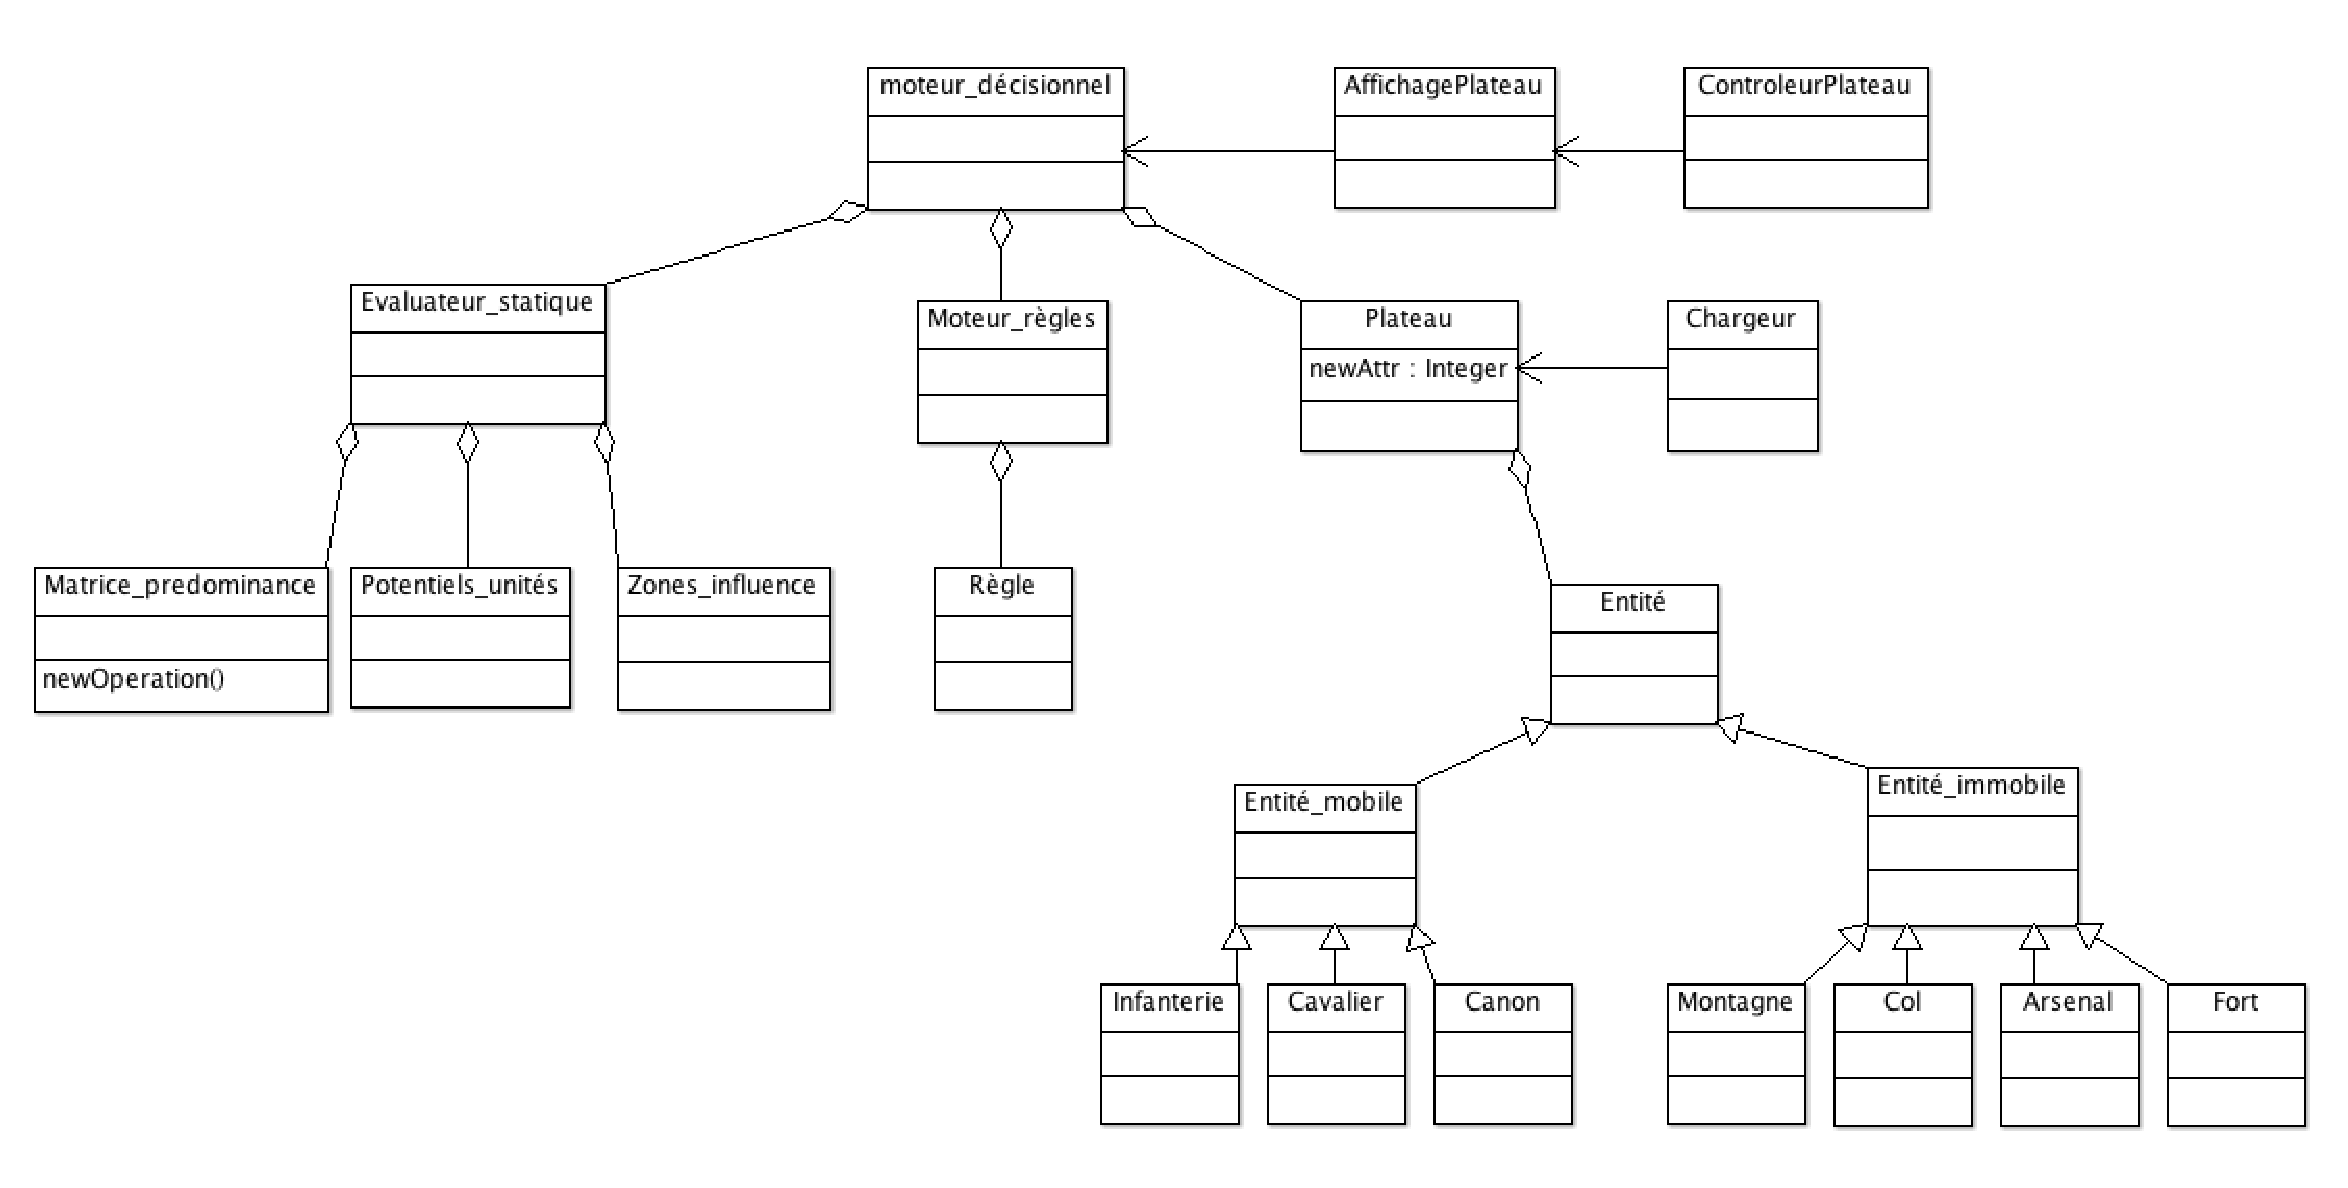
\includegraphics[scale=0.4]{images/diag_classes.eps}

			\clearpage

		\subsection{Description des classes}

			\subsubsection{Board}
			
				\paragraph{Définition :}
				Le Board est une matrice de taille fixe représentant une situation de jeu.
				\paragraph{Interaction :}
				Certaines cases du Board contiendront des objets de type Entity.
				

			\subsubsection{EntityLoader}

				\paragraph{Définition :}
				Classe permettant de charger une partie à partir d'un fichier. Elle transcrira les informations brute du 
				fichier en un Board contenant des Entity.
				\paragraph{Interaction :}
				L'EntityLoader interagira avec le Board puisque sa fonction consiste à modifier celui-ci.

			\subsubsection{Entity}

				\paragraph{Définition :}
				Les Entity représentent les éléments de jeu (les unités ainsi que les batiments et obstacles).
				\paragraph{Interaction :}
				Toutes les Entity seront disposées à l'intérieur d'une matrice dans la classe Board.

			\subsubsection{MovableEntity}

				\paragraph{Définition :}
				Les MovableEntity sont les unités movibles telles que les infanteries, les cavaliers, les canons ou toute autre unité 
				qu'il est possible de déplacer.
				\paragraph{Interaction :}
				Les MovableEntity seront disposées à l'intérieur d'une matrice dans la classe Plateau.

			\subsubsection{UnmovableEntity}

				\paragraph{Définition :}
				Les UnmovableEntity sont des entités présentes sur le plateau mais que les règles ne permettent pas de déplacer. 
				Les forts, les arsenaux, les montagnes ou les cols sont par exemple des UnmovableEntity.
				\paragraph{Interaction :}
				Les UnmovableEntity seront disposées à l'intérieur d'une matrice dans la classe Board. 
				Certaines UnmovableEntity pourront par ailleurs contenir des MovableEntity. (exemple : les forts)

			\subsubsection{Engine}

				!!!!!!!!!!!! A COMPLETER !!!!!!!!!!!!
				\paragraph{Définition :}
				Cette classe représente le moteur de règles et doit faire l'intermediaire entre les faits (la situation de jeu actuelle) 
				et les règles qui sont implémentées dans un fichier ".drl".
				\paragraph{Interaction :}
				L'Engine intéragira avec .....

			\subsubsection{Rule}

				!!!!!!!!!!!! A COMPLETER !!!!!!!!!!!!
				\paragraph{Définition :}
				Une règle sera une expression logique associée à un fait. Elles ne seront en fait pas codées sous forme de classe mais 
				sous forme de fichier en ".drl".
				\paragraph{Interaction :}
				Les règles seront envoyées à l'Engine qui devra se charger de les appliquer.

			\subsubsection{InfluenceArea}

				\paragraph{Définition :}
				Cette classe permettra de calculer les zones d'influence des unités, c'est à dire l'ensemble des cases sur lesquelles 
				chaque unité peut agir.
				\paragraph{Interaction :}
				La classe InfluenceArea aura besoin d'un objet de type Board pour faire ses calculs et stockera les résultats dans 
				les entités elles-mêmes.

			\subsubsection{Potential}

				\paragraph{Définition :}
				Cette classe permettra de calculer les potentiels offensifs et défensifs des unités en fonction de leur configuration spatiale.
				\paragraph{Interaction :}
				La classe Potential aura besoin d'un objet de type Board pour faire ses calculs et stockera les résultats dans les 
				entités elles-mêmes.

			\subsubsection{DangerousnessMatrix}

				!!!!!!!!!!!! A COMPLETER - Ne va même pas exister ? !!!!!!!!!!!!
				\paragraph{Définition :}
				Cette classe permettra de stocker la matrice de dangerosité représentant les endroit avantageux ou à éviter.
				\paragraph{Interaction :}
				La classe DangerousnessMatrix ...

			\subsubsection{StaticEvaluator}

				!!!!!!!!!!!! A COMPLETER - Ne va même pas exister ? !!!!!!!!!!!!
				\paragraph{Définition :}
				AREFAIRE : Le StaticEvaluator est la classe permettant de calculer et stocker l'ensemble des résultats de nos algorithme 
				d'évaluation statique du jeu.
				\paragraph{Interaction :}
				AREFAIRE : Le StaticEvaluator agit directement sur InfluenceArea, Potential et DangerousnessMatrix puisqu'il se charge 
				de les mettre à jour. Le moteur décisionnel aura quant à lui accès à l'évaluateur pour pouvoir prendre des décisions en fonction 
				des résultats trouvés par l'évaluateur.

			\subsubsection{DecisionnalEngine}

				\paragraph{Définition :}
				Le DecisionnalEngine se charge de choisir le coup à jouer en fonction d'une situation de jeu donnée et des résultats 
				du StaticEvaluator.
				\paragraph{Interaction :}
				Le DecisionnalEngine interagira avec le Board pour connaître la situation de jeu et les Entity pour connaître les 
				différentes données calculées par le StaticEvaluator.

		\clearpage
		
	\section{Choix algorithmiques}    

		\subsection{ A. gna gna}
		
		Ceci est du texte
		
		\subsection{ B. gna gna}
		
		Ceci est du texte
		
		\subsection{ C. gna gna}
		
		Ceci est du texte
		
		\clearpage
		
	\section{Tests réalisés}    

		\subsection{ A. gna gna}
		
		Ceci est du texte
		
		\subsection{ B. gna gna}
		
		Ceci est du texte
		
		\subsection{ C. gna gna}
		
		Ceci est du texte
		
		\clearpage
		
	\section{Difficultés rencontrées}    

		\subsection{ A. gna gna}
		
		Ceci est du texte
		
		\subsection{ B. gna gna}
		
		Ceci est du texte
		
		\subsection{ C. gna gna}
		
		Ceci est du texte
		
		\clearpage

	\section{Conclusion}
	
		Importer la biblio à la fin car chiant à générer sous latex.
		
		\clearpage

	\section{Elements bibliographiques}
	
		\begin{itemize}
		
		\item Le livre~\cite{ref1} présente une partie commentée du jeu de la guerre accompagnée de schémas illustrés. 
		De plus on peut trouver les règles officielles proposées par Guy Debord à partir de la page 131.
		\\[0.7\baselineskip]
		
		\item Le livre Artificial Intelligence for Games~\cite{ref2} aborde dans son 5\up{ème} chapitre la prise de décision d'un point de vue technique. 
		On y trouve le principe de fonctionnement et un exemple d'implémentation de diverses structures de données (arbre de décision, machine à état, 
		arbre de comportement, moteur de règles).
		\\[0.7\baselineskip]

		\item Ce site~\cite{ref3} regroupe l'ensemble des règles du jeu de la guerre et propose une version jouable. Cette version jouable permettra 
		de bien comprendre les règles du jeu et de vérifier que notre jeu a bien le même comportement.
		\\[0.7\baselineskip]
	
		\item Cet ouvrage~\cite{ref4} concernant l'intelligence artificielle propose une grande variété d'idées sur les programmes heuristiques. 
		Il explique comment gérer la prise de décision acceptable mais non optimale, dans les cas où la prise de décision optimale nécessite trop de ressources.
		\\[0.7\baselineskip]
		
		\item Cette page~\cite{ref5} propose des explications d'algorithmes utilisables dans le cas de jeu se jouant à deux, tour par tour et 
		pour lequel chaque joueur connait la position de son adversaire.
		\\[0.7\baselineskip]
		
		\item Cette page~\cite{ref6} propose un tutoriel très complet sur l'utilisation de Jboss drools, outil qui nous permettra de concevoir notre moteur de règles.
		\\[0.7\baselineskip]
		
		\item Ce tutoriel~\cite{ref7} sur la bibliothèque Swing pourra nous servir pour la conception de l'interface graphique. Cette bibliothèque 
		permettra par exemple d'afficher le plateau et d'interagir avec au besoin.
		\\[0.7\baselineskip]
		
		\end{itemize}
		
		\bibliographystyle{unsrt}
		\bibliography{ref.bib}{}

\end{document}                                 
